\let\negmedspace\undefined
\let\negthickspace\undefined
\documentclass[journal]{IEEEtran}
\usepackage[a5paper, margin=10mm, onecolumn]{geometry}
%\usepackage{lmodern} % Ensure lmodern is loaded for pdflatex
\usepackage{tfrupee} % Include tfrupee package

\setlength{\headheight}{1cm} % Set the height of the header box
\setlength{\headsep}{0mm}     % Set the distance between the header box and the top of the text

\usepackage{gvv-book}
\usepackage{gvv}
\usepackage{cite}
\usepackage{amsmath,amssymb,amsfonts,amsthm}
\usepackage{algorithmic}
\usepackage{graphicx}
\usepackage{textcomp}
\usepackage{xcolor}
\usepackage{txfonts}
\usepackage{listings}
\usepackage{enumitem}
\usepackage{mathtools}
\usepackage{gensymb}
\usepackage{comment}
\usepackage[breaklinks=true]{hyperref}
\usepackage{tkz-euclide} 
\usepackage{listings}
% \usepackage{gvv}                                        
\def\inputGnumericTable{}                                 
\usepackage[latin1]{inputenc}                                
\usepackage{color}                                            
\usepackage{array}                                            
\usepackage{longtable}                                       
\usepackage{calc}                                             
\usepackage{multirow}                                         
\usepackage{hhline}                                           
\usepackage{ifthen}                                           
\usepackage{lscape}


\renewcommand{\thefigure}{\theenumi}
\renewcommand{\thetable}{\theenumi}
\setlength{\intextsep}{10pt} % Space between text and floats

\numberwithin{equation}{enumi}
\numberwithin{figure}{enumi}
\renewcommand{\thetable}{\theenumi}	

% Marks the beginning of the document
\begin{document}
\bibliographystyle{IEEEtran}

\title{9-9.5-4}
\author{EE24BTECH11049 \\ Patnam Shariq Faraz Muhammed}

% \maketitle
% \newpage
% \bigskip
{\let\newpage\relax\maketitle}

\textbf{QUESTION:} \\
	Find the area of the region \cbrak{\brak{x, y} : y^2 \leq 4x, 4x^2 + 4y^2 \leq 9} , using integration.\\
\textbf{SOLUTION:} \\
	\begin{table}[h!]    
		\centering
		\begin{tabular}[12pt]{ |c| c| c|}
\hline
\textbf{Variables} & \textbf{Description} & \textbf{Formula} \\
\hline
$A$ & A point in the 2-D plane whose coordinates are as follows & $\brak{k + 1, 2k}$\\
\hline
$B$ & A point in the 2-D plane whose coordinates are as follows & $\brak{3k, 2k + 3}$\\
\hline
$C$ & A point in the 2-D plane whose coordinates are as follows & $\brak{5k − 1, 5k}$\\
\hline
\end{tabular}

		\label{table: 9-9.5-4}
	\end{table}\\

	The general equation of a parabola with directrix $\vec{n}^{\top}\vec{x}=c$ is given by,
	\begin{align*}
		g\brak{\vec{x}}=\vec{x}^{\top}\vec{V}\vec{x}+2\vec{u}^{\top}\vec{x}+f=0\\
		\vec{V}=\norm{\vec{n}}^2\vec{I}-e^2\vec{n}\vec{n}^{\top}\\
		\vec{u}=ce^2\vec{n}-\norm{\vec{n}}^2\vec{F}\\
		f=\norm{\vec{n}}^2\norm{\vec{F}}^2-c^2e^2
	\end{align*}
	for the parabola $y^2=4x$, equation of directrix is, $\myvec{1&0}\vec{x}=-1$
	\begin{align*}
		\vec{V}&=\myvec{0&0\\0&1}\\
		\vec{u}&=\myvec{-2\\0}\\
		f&=0
	\end{align*}
	The given circle can be expressed as conics with parameters
	\begin{align*}
		\vec{V}&=\frac{1}{4}\myvec{9 & 0\\0 & 9}\\
		\vec{u}&=0\\
		f&=-\frac{81}{16}
	\end{align*}

	The intersection of two conics with parameters $\vec{V}_i,\vec{u}_i,f_i, i=1,2$ is defined as,
	\begin{align*}
		\vec{x}^{\top}\brak{\vec{V_1}+\mu\vec{V_2}}\vec{x}+2\brak{\vec{u_1}+\mu\vec{u_2}}^{\top}\vec{x}+\brak{f_1+\mu f_2}&=0\\
		\mu&=-\frac{4}{9}\\
	\end{align*} 
	On solving we get the points of intersection to be $\myvec{\frac{1}{2}\\\sqrt{2}}, \myvec{\frac{1}{2}\\-\sqrt{2}}$\\
	
	The desired area of region is given as\\
	\begin{align*}
		&= 2\sbrak{\int_{0}^{\frac{1}{2}} 2\sqrt{x} \, dx + \int_{\frac{1}{2}}^{\frac{3}{2}} \sqrt{\frac{9}{4}-x^2} \, dx}\\
		&= 2\sbrak{\frac{4}{3}\sqrt{x^3}}_0^\frac{1}{2} + 2\sbrak{\frac{x}{2}\sqrt{\frac{9}{4}-x^2} + \frac{9}{8}\sin^{-1}\brak{\frac{2x}{3}}}_\frac{1}{2}^\frac{3}{2}\\
		&= \frac{9\pi}{16}-\frac{1}{2\sqrt{2}}-\frac{9}{8}\sin^{-1}\brak{\frac{1}{3}}
	\end{align*}\\
	\begin{figure}[ht]
		\centering
		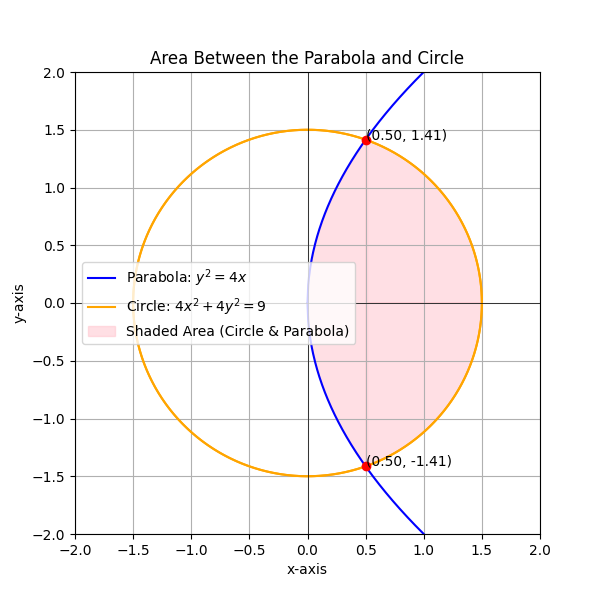
\includegraphics[width=0.8\textwidth]{figs/fig.png}
		\caption{A plot of the given question.}
	\end{figure}
\end{document}
